% !TeX document-id = {adfd8c77-9aa9-43e7-acaa-af378587f0c7}
% !TeX TXS-program:compile = txs:///pdflatex/[--shell-escape]
\documentclass{article}

\usepackage[utf8]{inputenc}
\usepackage[T1]{fontenc}
\usepackage{color}
\usepackage{soul}
\usepackage{amsmath}
\usepackage{amssymb}
\usepackage{listings}
\usepackage{minted}
\usepackage{hyperref}
\usepackage{graphicx}
\usepackage{calc}
\usepackage{enumitem}
\usepackage{standalone}

\usepackage{tikz}
\usetikzlibrary{datavisualization}
\usetikzlibrary{datavisualization.formats.functions}

\graphicspath{{img/}}
\setlength{\parindent}{0pt}

\begin{document}

\title{CW 19 summary}
\author{Alexander Pastor}
\date{04.05.2017}
\maketitle
\tableofcontents
\newpage

\section{Understanding RF Specifications}

\subsection{Basic Terminology}

\emph{Digitizer Amplitude Error}

The following formula provides the dampening or attenuation factor E of the digitizer:

\begin{equation}
	E = 1- \frac{R}{\sqrt{1+R^2}}
\end{equation}

\medskip

A X-Hz digitizer is defined to have $ E = \frac{1}{\sqrt{2}}$ at the frequency X, which implies $R=1$ for the frequency X. X is called bandwidth of the digitizer in this context, and R is the ratio of the digitizer bandwidth and the maximum frequency of interest $\frac{f_d}{f_i}$.

\begin{figure}[h]
	\centering
	\label{amplitude_error}
	\documentclass[border=2mm,tikz]{standalone}
\usepackage{tikz}
\usetikzlibrary{datavisualization}
\usetikzlibrary{datavisualization.formats.functions}
\begin{document}
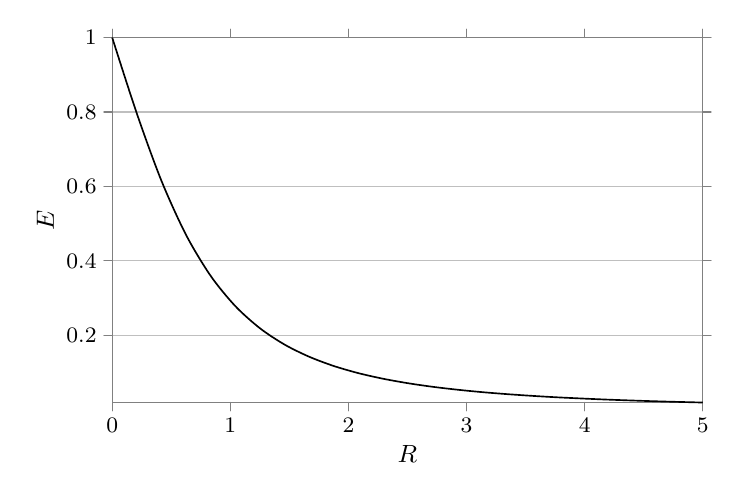
\begin{tikzpicture}
\datavisualization [scientific axes,
					y axis=grid,
                    y axis={label={$E$}},
                    x axis={label={$R$}},
                    visualize as smooth line,
                    scale = 1.5
                   ]

data [format=function]
{
  var x : interval [0:5];
  func y = 1 - ((\value x)/(sqrt(1 + \value x * \value x)));
};
\end{tikzpicture}
\end{document}
	\caption{Digitization error verus bandwidth ratio}
\end{figure}

It is recommended by NI to have X be 3 to 5 times higher than the frequency of interest. This corresponds to errors or dampening between 1.94\% and 5.13\% 

\bigskip

\emph{Rise Time}

Rise time is defined as the time a signal needs to rise from 10\% to 90\% of its steady-state or periodic maximum.

\bigskip

\begin{itemize}
	\item The rise time of a simple RC-circuit is about $\frac{0.35}{RC}$.
	\item The formula to calculate the total rise time of a digitized signal is: $$ T_{r_t} = \sqrt{{T_{r_s}}^2 + {T_{r_d}}^2}$$
	\item In order to minimize rise time errors NI recommends to have $T_{r_d}$ be around $\frac{1}{3}$ and $\frac{1}{5}$ of $T_{r_s}$.
\end{itemize}

\emph{Nyquist Theorem}

The bandwidth of the digitizer must be at least 2 times the maximum frequency of the signal to avoid aliasing. 

\medskip

$\Leftrightarrow$ To extinguish aliasing in the passband one either has to make sure the Nyquist Theorem is matched or apply a lowpass filter to limit the signal's bandwidth.

\bigskip

\emph{Phase Noise}

\bigskip

\emph{Resolution Bandwidth}

\bigskip

\emph{Noise Density}

\bigskip

\emph{Dynamic Range}

\bigskip

\emph{Voltage Standing Wave Ratio (VSWR)}

\bigskip

\emph{Frequency Response}

\bigskip
 
\emph{Modulation Error Ratio (MER)}

\bigskip

\emph{Error Vector Magnitude (EVM)}

\bigskip

\emph{Third-Order Intercept (TOI)}

\section{Physical Layer Challenge}

\section{Good to Know...}

\subsection{Python}

\subsection{\LaTeX}

I learned...

\begin{itemize}
	\item ... when to use \href{https://tex.stackexchange.com/questions/246/when-should-i-use-input-vs-include}{input or include}
	\item ... some tikz basics
\end{itemize}

\end{document}